\documentclass[11pt]{article}
\usepackage{multirow}
\usepackage[headings]{fullpage}
\usepackage{url}
\usepackage{color}
\usepackage{graphicx} 
\usepackage{float}
\usepackage[dvipsnames]{xcolor}
\usepackage{fancyhdr}
\usepackage{lastpage}
\usepackage{longtable}

\newcommand{\grads}{GRaDs}
\newcommand{\mn}{MareNostrum}
\newcommand{\mg}{MapGenerator}
\newcommand{\kw}[1]{{\textbf{#1}}}
\newcommand{\todo}[1]{\color{red}{#1}\color{black}}

\pagestyle{fancy}
\fancyhead{}
\fancyfoot{}
\fancyhead[LO,RE]{\raisebox{-0.5\height}{\includegraphics[width=3cm]{bsc_style/bsc_h_ul.pdf}}\vspace{2pt}\\ \sffamily\scriptsize\color{Blue}\textbf{Earth Sciences Department\\Departamento de Ciencias de la Tierra}}
\fancyhead[C]{\Large{\textbf{{\color{Blue}Proyecto CALIOPE\\Generaci\'on de im\'agenes}}}}
\fancyhead[RO,RE]{\raisebox{.75\height}{\parbox{3.5cm}{\sffamily\footnotesize\color{Blue}\textbf{Date}: 19 de abril del 2011\\\textbf{Page}: \thepage~of \pageref{LastPage} \\\textbf{Code:}}}}
\fancyfoot[LO,RE]{\small\color{Blue}\begin{tabular}{p{4cm}}\textbf{Written by}: Luca Telloli \\ \textbf{Date:} \today\end{tabular}}
\fancyfoot[C]{\small\color{Blue}\begin{tabular}{p{3cm}}\textbf{Reviewed by}: \\ \textbf{Date:}\end{tabular}}
\fancyfoot[RO,RE]{\small\color{Blue}\begin{tabular}{p{3.5cm}}\textbf{Approved by}: \\ \textbf{Date:}\end{tabular}}
\renewcommand{\footrulewidth}{.5pt}
\addtolength{\headheight}{2\baselineskip}


\begin{document}

\title{\mg{}: a wrapper for GraDs images around the Matplotlib plotting engine}
\author{Luca Telloli}
\date{}
\maketitle

\tableofcontents 
\section{Introduction} 
Historically, a collection of independent \grads{} scripts have been using inside the Caliope workflow to produce images of air-quality, emissions and meteorology from the output of simulations. As the number of simulated domains has grown and evolved into a larger collection of domain and subdomains, the usual copy-and-paste for the GraDs code rendered a collection of similar scripts with small differences and costly maintenance. 

\mg{} is an attempt to resolve this issue programmatically by producing a reusable code driven by a simple, human-readable, text-only configuration file. 

\subsection{General description of the software}
\mg{} is a Python software for generating images. The software reads data from one or more data sources (in the form of a data file, typically in netCDF format), and visualizes them onto a .gif image for one or more time steps. Additionally, the software produces an animated image by aggregating all the static images in the output directory into an animated .gif. 

Inside the Caliope workflow, the software is currently used every day, after the CMAQ simulation of each domain, to produce air-quality and emissions images. There are currently 27 ``packs'' of images; one for the EU domain, one for the Iberian Peninsula + one for each of its 15 regions, one for Andalusia and one for Canary Island + one for each of its 7 islands. A total of 11 contaminants (5 for Air Quality + 6 for Emissions) is run for each pack, and for each contaminant 49 images are generated, plus a .gif animation, for a total of 14553 images and 297 animations. 

\section{Installation \& Configuration}
The source code of \mg{} can be downloaded from the BSC svn server, at the following path: 
\url{https://svn.bsc.es/repos/earth/sds-was/mapgenerator/branches/caliope}. 

\subsection{Pre-requisites} 
\label{ssec:prereq}
The libraries have some prerequisites that should be met: 
\begin{itemize}
\item a version of python 2.6.x or higher 
\item Matplotlib (v. 1.0.1), an open-source plotting library in python (\url{http://matplotlib.sourceforge.net/}) and the Basemap toolkit
\item GaLab (v. 1.0.1), an open-source python interface to GraDs 
\item Grads (v. 2.0.a9), an interactive desktop tool that provides access, manipulation, and visualization capabilities of earth science data (\url{http://www.iges.org/grads/})
\item the ImageMagick software suite (v.6.3.5 or higher, \url{http://www.imagemagick.org/}) 
\end{itemize} 

In particular, the current \texttt{PATH} environment variable should be up to date to include the Grads executable. On \mn{}, the \url{run_mn.sh} script takes care of this issue. 

\subsection{Architecture} 
Figure \ref{fig:arq} shows the software stack of the application. 

\begin{figure}[H]
\begin{center}
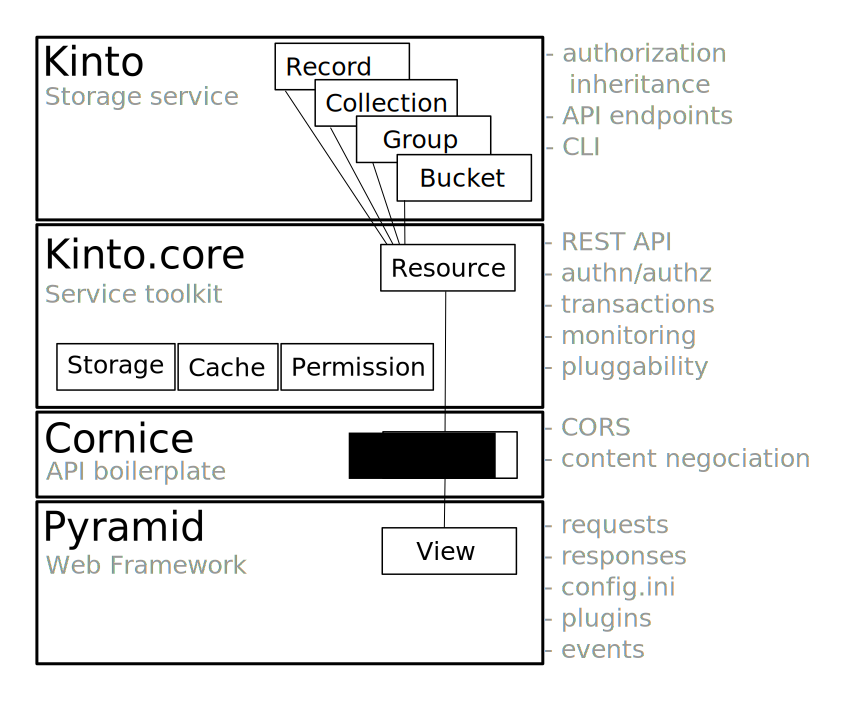
\includegraphics[width=.65\textwidth]{img/architecture.pdf}
\end{center}
\caption{Architecture of \mg{}}
\label{fig:arq}
\end{figure}

At the bottom level, the application uses GraDs, through the GaLab wrapper, to retrieve data from the input files. \grads{} can not only handle simple variables, but also resolve more complex mathematical expressions. 

Once the data have been retrieved, Basemap is taking care of the drawing part; finally, some additional layers of information to display use Matplotlib APIs. 

\subsection{General workflow}
Figure \ref{fig:wflow} shows the general workflow of the application. 

\begin{figure}[H]
\begin{center}
\includegraphics[height=0.7\textheight]{img/gflow.pdf}
\end{center}
\caption{Architecture of \mg{}}
\label{fig:wflow}
\end{figure}

\section{Usage}
The main executable for image generation is the \url{map_main.py} file, located inside the \url{bin} directory of the main distribution; this file expects at least one parameter which identifies the section to generate inside a configuration. 
Additionally, a different configuration file from the default one can be specified with the \texttt{-c} option.

For instance, the command: 
\begin{center}
\begin{verbatim}
python map_main.py -c example.conf Section1 
\end{verbatim}
\end{center}
will look for \texttt{[Section1]} inside the file \url{example.conf}, read the configuration and generate the corresponding images. 


\subsection{Configuration files}
Configuration files contain all the information needed for a run; here the user can specify information such as input directories, output directories, output map coordinates (latitude and longitude), total number of output images and their dpi, some image's attributes such as image resolution, wind's density, etc. 

Appendix \ref{app:conf-file} shows an example of a configuration file, which is a simple text-only file. Each file is divided into sections, starting with a label specified between square brackets, plus a \texttt{General} section specifying values common to all sections. Each value is specified in the form \texttt{key = value}. A list of keys and expected values is provided in appendix \ref{app:keyval}. 

Each section can override values from the \texttt{General} section by simply providing a new value for the same keyword. Finally, most values inside a configuration file can be overridden directly from the command line. 

\subsection{Data sources and descriptors}
The keyword \kw{srcfile} specifies a list of one or more data sources; these files will be processed by the \grads{} engine  by evaluating the expression of the corresponding entry of the \kw{var} keyword. 

The data source should be a self-contained source, which specifies all the data \grads{} need to draw it directly. Most of the time, this won't be true so instead of specifying a NetCDF file, the user can specify a descriptor file which contains directives that help \grads{} in the correct interpretation of the input data. Appendix \ref{sec:grads-descriptor} provides an example of such a descriptor file; for further details refer to \url{http://www.iges.org/grads/gadoc/descriptorfile.html}

\section{Running on MareNostrum}

\subsection{Generating images}

The \url{scripts} subdirectory contains a script called \url{run_mn.sh} which facilitates most of the tasks for a run on \mn{}.

The script assumes the following directory structure: 
\begin{verbatim}
\__
   \bin__
         \current [-> symlink to releases/rXXX, where XXX is the release in use]
   \releases 
   \run_mn.sh     [-> symlink to bin/current/scripts/run_mn.sh]
   \check_out.sh  [-> symlink to bin/current/scripts/check_out.sh]
\end{verbatim}
 
The \url{run_mn.sh} script requires 4 parameters: 
\begin{description}
\item[date]: date to simulate, in the YYYYMMDD format 
\item[domain]: domain to simulate, see figure \ref{fig:domains}
\item[subdomain]: the subdomain to simulate,  see figure \ref{fig:domains}
\item[class]: type of images, currently `aq', `emis' or `meteo'; see figure \ref{fig:domains}
\end{description}

For each domain/subdomain/class, the script expects a file named \textit{class}/\textit{domain}.\textit{subdomain}.conf inside the \url{conf} directory and tried to execute all the sections inside the given configuration file in their order of appeareance. 

The script is configured to run on \mn{}, with some predefined execution paths. 
In particular, the following directories are assumed to be valid: 
\begin{enumerate}
\item \url{/gpfs/apps/IMAGEMAGICK/6.7.3-5/bin/} \& \url{/gpfs/apps/GRADS/2.0.a9/bin/}, used inside the \texttt{PATH} variable 
\item \url{/gpfs/apps/PYTHON/2.7.1/32/bin/python}, which is the release of python in use, including the necessary required libraries (see \ref{ssec:prereq})
\item \url{/gpfs/projects/bsc32/bsc32359/CMAQ-mat/FORECAST/AQ/IMG}, the initial directory where to run 
\item \url{/gpfs/projects/bsc32/bsc32359/CMAQ-mat/FORECAST/}, the directory where input data are located 
\end{enumerate}

Figure \ref{fig:domains} shows the domains subdomains and classes currently supported by the application. 

\begin{figure}[H]
\begin{center}
\includegraphics[height=0.55\textheight]{img/domains.pdf}
\end{center}
\caption{Domains}
\label{fig:domains}
\end{figure}

The currently supported options by the \texttt{run\_mn.sh} script are: 
\begin{verbatim}
Usage: 
run_mn.sh [-abcdopr] DATE DOMAIN SUBDOMAIN CLASS
  DATE in YYYYMMDD format
  CLASS in {aq, emis, meteo}

OPTIONS:
  -a:	Additional arguments to pass to the python executable
  -b:	Set basedir to given value
  -c:	Set configuration dir to given value
  -C:	Create configuration files only (inside current directory)
  -d:	Set data dir base to given value
  -o:	Set out dir base to given value
  -p:	Use the given python executable
  -r:	Use specified release
  -s:	Use specified source dir
  -S:	Match string
\end{verbatim}

\subsubsection{Example}
Invoking the following command:
\begin{verbatim}
run_mn.sh 20111210 ip ip aq
\end{verbatim}
will run an execution for all sections inside the \url{aq/ip.ip.conf} file inside the \url{conf} directory. 

\subsubsection{Example}
One useful option is the \texttt{-S} option which can be used to match a specific contaminant. Invoking the following command: 
\begin{verbatim}
run_mn.sh -s PM10_DUST 20111210 ip ip aq
\end{verbatim}

will only run the section inside the configuration file that matches the regular expression \texttt{*PM10\_DUST}. If no section matches this value, nothing will be run. 

\subsubsection{Example}
Invoking the following command:
\begin{verbatim}
run_mn.sh -o /tmp/test 20111210 ip ip aq
\end{verbatim}
will run an execution for all sections inside the \url{aq/ip.ip.conf} file inside the \url{conf} directory and will place the output inside the \url{/tmp/test} directory. The path provided to the command are \textbf{expected to be absolute}.

\subsection{Checking the generated output}
\label{ssec:check-out}
The \url{scripts} directory contains another script named \url{check_out.sh} which purpose is to check if all packs of images were correctly produced, and relaunch any pack that was not created nor completed. 

The currently supported options of the \url{check_out.sh} script are: 
\begin{verbatim}
Usage: check_out.sh [-c CLASS] [-f] [-w] [DATE]
optional DATE parameter to specify a custom date, otherwise today
    -c: CLASS argument to choose in 'aq', 'emis' or 'meteo'
    -f: fix missing images (launches a job on MN)
    -w: use current directory as base dir
\end{verbatim}

Note: if a class is not specified, the 'aq' class is assumed as the default class. 

\subsubsection{Example}
Invoking the following command: 
\begin{verbatim}
check_out.sh -f 
\end{verbatim}

will check if all air quality images have been produced, and will launch a job on MareNostrum for each pack that was not correctly generated. 

\subsubsection{Example}
Invoking the following command: 
\begin{verbatim}
check_out.sh -c emis
\end{verbatim}

will check if all images of the 'Emissions' class have been generated. At the end it will display a report for each pack that was generated or missing. Appending the \texttt{-f} flag would also force the regeneration of any missing pack. 

\subsection{Control script}
The generation of images for CALIOPE is started from the control script, a C-shell script located in \url{/gpfs/projects/bsc32/bsc32359/CMAQ-mat/FORECAST/AQ/scripts/} and named \url{control_global.sc}. 

Currently, the generation of each pack of images is started right after the finalization of the simulation producing the input data. For instance, the images for the Iberian Peninsula are generated with the following commands: 
\begin{verbatim}
foreach p ( ip andalucia aragon asturias baleares cantabria \
            castillalamancha castillaleon catalunya extremadura \
            galicia larioja madrid murcia navarra paisvasco valencia )
        $JOBIFY -n im_aq_${p} -w1h  -a es1 -c benchmark -i $IMG_NEW \
            -l logs/$YEARMONTHDAY ./run_mn.sh $YEARMONTHDAY IP ${p} aq
        $JOBIFY -n im_em_${p} -w90m -a es1 -c benchmark -i $IMG_NEW \
            -l logs/$YEARMONTHDAY ./run_mn.sh $YEARMONTHDAY IP ${p} emis
end
\end{verbatim}

At the end of the script, a control is placed to check if all images were properly created, using the script in section \ref{ssec:check-out}, with the following commands: 
\begin{verbatim}
$IMG_NEW/check_out.sh -f
$IMG_NEW/check_out.sh -f -c emis 
\end{verbatim}

The following environment variables are used:
\begin{description}
\item[JOBIFY]: path to the jobify.sh script, a script used to submit any script as a job for \mn{}. The current value of this variable is \url{/gpfs/projects/bsc32/share/bin/jobify.sh}
\item[IMG\_NEW]: the base directory where the software distribution is installed. The current value of this variable is \url{/gpfs/projects/bsc32/bsc32359/CMAQ-mat/FORECAST/AQ/IMG}
\item[YEARMONTHDAY]: specifies the simulation date with a YYYYMMDD pattern
\end{description}

\section{Improvements over previous version}
The use of this software adds some relevant improvements to the original, \grads{}-only software, including: 
\begin{description}
\item[higher quality images]: the quality of images improved with more deepness (due to the increase in the number of colors) and anti-aliasing support (improves the appearance of polygon edges, especially in typographic characters)
\item[substantial reduction of code size]: instead of copies of similar code running for each domain/subdomain, there is now a single code and multiple, compact configuration files which express domain-specific characteristics. The \grads{} scripts comprised around 1500 lines of code for each pack, while the new code is about 1000 lines, plus about 80 to 100 lines for each pack's configuration file, implying a reduction of more than 90\% in the total number of lines. 

\item[rationalization of the process]: 
\begin{itemize}
\item configuration files are organized in directories with meaningful names
\item images are organized in \emph{packs} (one pack for each domain/subdomain)
\item output directory is organized in a hierarchical tree by date, class, domain and subdomain 
\item image elements (maps, colorbars, titles) and their positioning are now consistent thorough all packs 
\end{itemize}

\item[smaller animations]: with the use of ImageMagick operators, the size of animations has been reduced from 30\% up to 70\%

\item[higher granularity]: the code allows for the creation of any item of a sequence of images, or a specific pack, or all images of a domain. All values are overridable from command line
\item[other graphical improvements], which include: 
	\begin{itemize}
	\item configurable support for winds and wind arrows densities
	\item configurable support for image proportions 
	\item configurable support for air quality limits 
	\end{itemize}
\end{description}

\subsection{Performance}
Table \ref{t:times-aq} provides a view of the current running times for Air Quality image generation, while \ref{t:times-em} provides information for Emissions image generation. Previous running times for Air Quality have been quantified as ``more or less'' 30 to 40 minutes for each pack, including all contaminants; no quantification was previously provided for Emissions' images. The new application allows a better granularity, providing precise times for each contaminant. 

From tables \ref{t:times-aq}, we can deduce that the general level of performance on MareNostrum (where each pack runs in parallel) has been maintained, while the single pack performance has been maintained or improved. 

\begin{table}
\begin{center}
\begin{tabular}{lllllll}
DOMAIN & O3 & NOx & SO2 & CO & PM10 & TOTAL \\
\hline\hline
eu & 4.8 & 4.7 & 4.3 & 4.2 & 18.0 & 35.9\\
ip & 6.2 & 6.9 & 6.7 & 6.5 & 14.2 & 40.4\\
andalucia & 5.6 & 5.9 & 5.9 & 5.7 & 7.6 & 30.7\\
aragon & 5.6 & 5.7 & 5.8 & 5.9 & 7.6 & 30.5\\
asturias & 5.5 & 5.6 & 5.8 & 5.7 & 6.9 & 29.4\\
baleares & 2.5 & 2.5 & 2.4 & 2.3 & 4.5 & 14.1\\
cantabria & 5.5 & 5.7 & 5.8 & 5.6 & 6.7 & 29.2\\
castillalamancha & 5.6 & 6.2 & 6.0 & 5.9 & 7.6 & 31.2\\
castillaleon & 5.8 & 6.2 & 6.1 & 6.0 & 8.0 & 32.0\\
catalunya & 5.5 & 5.9 & 5.8 & 5.7 & 7.5 & 30.2\\
extremadura & 5.5 & 5.8 & 5.7 & 5.5 & 7.3 & 29.8\\
galicia & 5.5 & 5.9 & 5.7 & 5.5 & 7.2 & 29.8\\
larioja & 5.6 & 5.6 & 5.5 & 5.6 & 6.8 & 29.1\\
madrid & 5.4 & 5.6 & 5.5 & 5.6 & 6.8 & 28.9\\
murcia & 5.4 & 5.8 & 5.6 & 5.5 & 7.3 & 29.6\\
navarra & 5.1 & 5.4 & 5.3 & 5.2 & 6.6 & 27.5\\
paisvasco & 5.5 & 6.0 & 5.7 & 5.8 & 7.2 & 30.2\\
valencia & 5.4 & 5.9 & 5.7 & 5.8 & 7.2 & 30.0\\
canarias & 3.2 & 3.1 & 3.2 & 3.2 & 9.4 & 22.1\\
tenerife & 2.3 & 2.5 & 2.4 & 2.2 & 3.5 & 12.9\\
grancanaria & 2.3 & 2.4 & 2.2 & 2.2 & 3.6 & 12.6\\
fuerteventura & 2.3 & 2.4 & 2.2 & 2.2 & 3.6 & 12.6\\
lanzarote & 3.8 & 3.7 & 3.7 & 3.7 & 4.9 & 19.7\\
lagomera & 3.6 & 3.6 & 3.7 & 3.6 & 4.7 & 19.3\\
lapalma & 3.6 & 3.6 & 3.5 & 3.5 & 4.5 & 18.6\\
elhierro & 3.7 & 3.5 & 3.5 & 3.5 & 4.5 & 18.7\\
bcn & 4.2 & 4.6 & 4.2 & 4.3 & 9.8 & 27.1\\\end{tabular}
\end{center}
\label{t:times-aq}
\caption{Running times (in minutes) for Air Quality images (data from Jan, 8th 2012 run)}
\end{table}

\begin{table}
\begin{center}
\begin{tabular}{llllllll}
DOMAIN & NO & NO2 & SO2 & PM & CO & VOCs &TOTAL\\
\hline\hline
eu & 11.4 & 10.4 & 12.8 & 31.9 & 11.2 & 27.4 &104.9\\
ip & 9.9 & 10.0 & 10.3 & 22.3 & 10.8 & 30.9 &94.1\\
andalucia & 6.2 & 6.3 & 6.8 & 8.9 & 6.9 & 11.9 &47.0\\
aragon & 5.9 & 6.0 & 6.2 & 8.4 & 6.5 & 9.8 &42.6\\
asturias & 5.3 & 5.3 & 5.4 & 7.1 & 5.7 & 8.1 &36.9\\
baleares & 5.3 & 5.2 & 5.5 & 7.1 & 5.4 & 8.5 &36.9\\
cantabria & 5.6 & 5.6 & 5.7 & 7.3 & 5.6 & 8.4 &38.1\\
castillalamancha & 6.2 & 6.4 & 6.3 & 9.1 & 6.6 & 11.0 &45.6\\
castillaleon & 6.5 & 6.8 & 6.7 & 9.6 & 7.0 & 11.2 &47.7\\
catalunya & 5.8 & 6.1 & 6.0 & 7.5 & 6.1 & 9.7 &41.1\\
extremadura & 5.3 & 5.5 & 5.6 & 7.9 & 5.9 & 10.1 &40.1\\
galicia & 5.9 & 5.9 & 6.0 & 8.1 & 6.3 & 8.9 &40.9\\
larioja & 5.3 & 5.4 & 5.4 & 7.2 & 5.7 & 8.3 &37.2\\
madrid & 5.4 & 5.7 & 5.7 & 7.1 & 5.7 & 9.1 &38.8\\
murcia & 5.2 & 5.2 & 5.2 & 7.2 & 5.4 & 8.9 &37.1\\
navarra & 5.6 & 5.7 & 5.7 & 7.7 & 5.9 & 8.9 &39.5\\
paisvasco & 5.8 & 5.9 & 5.9 & 7.5 & 6.1 & 8.1 &39.3\\
valencia & 5.6 & 5.8 & 5.7 & 7.9 & 5.8 & 9.3 &40.1\\
canarias & 4.6 & 4.5 & 4.4 & 13.6 & 5.0 & 20.4 &52.5\\
tenerife & 3.2 & 3.1 & 2.5 & 3.8 & 3.3 & 4.7 &20.5\\
grancanaria & 3.0 & 2.8 & 2.4 & 3.6 & 3.1 & 4.3 &19.0\\
fuerteventura & 3.9 & 3.8 & 3.6 & 4.7 & 4.2 & 5.2 &25.4\\
lanzarote & 3.8 & 3.8 & 3.6 & 4.2 & 4.1 & 4.8 &24.3\\
lagomera & 3.7 & 3.6 & 3.5 & 4.2 & 4.0 & 5.0 &23.9\\
lapalma & 3.6 & 3.5 & 3.4 & 4.1 & 3.8 & 4.9 &23.2\\
elhierro & 3.5 & 3.2 & 3.2 & 4.0 & 3.5 & 4.6 &21.9\\
bcn & 5.6 & 5.5 & 5.5 & 14.6 & 5.9 & 21.6 &58.6\\
\end{tabular}
\end{center}
\label{t:times-em}
\caption{Running times (in minutes) for Emissions images (data from Jan, 8th 2012 run)}
\end{table}

\appendix
\section{List of configurable attributes}
\label{app:keyval}
\footnotesize
\begin{longtable}{lp{3.5cm}p{5.5cm}p{4cm}}
\hline
\multicolumn{4}{l}{\textbf{General values}}\\
\hline
Name & Type & Description &	Example\\
\hline\hline
\texttt{indir}	& string			& input directory, where data files are located & indir = .\\
\texttt{outdir} & string			& output directory, where images will be placed & outdir = out\\
lat 			& list of floats	& lower latitude, upper latitude, distance between lines & lat = 41.6, 44.0, 0.2\\
lon 			& list of floats	& lower longitude, upper longitude, distance between lines & lon = -9.7, -6.3, 0.3\\
max				& list of ints		& time steps where image of max should be printed & max = 23, 47\\
total			& int				& number of images to draw 					& total = 49\\
start			& int				& starting time step 					& start = 0\\
interval		& int				& time steps between two consecutive images	& interval = 1\\
srcfile			& list of strings	& list of input data files (or data descriptor files) & srcfile = pollutants.sdf,\\
var				& list of strings	& list of variables to draw. Accepts any formula supported by GraDs & var = 'o3*1962'\\
gap				& list of ints		& list of the first time step to take from each specified source. Useful when multiple input data have different initial times. Size of this list and srcfile should be equal & gap = 1, 13\\
bounds			& list of float		& list of values for value intervals in the image drawing & bounds = 0.1, 0.15, 0.2, 0.3, 0.4, 0.5, 0.65, 0.8, 1, 1.5, 2, 3, 4, 5\\
\hline
\multicolumn{4}{l}{\textbf{Drawing values}}\\
\hline
Name & Type & Description &	Example\\
\hline\hline
resolution		& value in: \{`l', `i', `h', `f'\}		& map resolution. Higher resolutions require higher initialization times & resolution = `l'\\
limits			& list of int							& drawing of black triangles at the configured levels & limits = 120, 180, 240\\
under			& HTML color string						& color for values below first in bounds & under = `\#004BFF'\\
over			& HTML color string						& color for values above last in bounds  & over  = `\#000000'\\
colors 			& list of HTML color strings			& list of colors to apply over the bounds list. 
The two lists should have the same size & colors = `\#075aff', `\#1f9df0', `\#2bffe5', ...\\
area\_thresh	& int									& threshold for drawing surfaces. Any surface with an area smaller than the specified value won't be represented. Value is in km$^2$ & area\_thresh = 100\\
colorbar		& boolean								& boolean toggle for colorbar. Default: true & colorbar = False\\
\hline
\multicolumn{4}{l}{\textbf{Optional drawing values}}\\
\hline
Name & Type & Description &	Example\\
\hline\hline
shapes			& list of strings						& list of additional shapefiles to draw on the picture. The files should be placed into the INDIR/data directory & shapes = `ESP\_adm1', `ESP\_adm2',\\
drawopts		& any subset of strings from \{`coastlines', `countries'\} & draw additional graphical elements on the map & drawopts = 'coastlines'\\
wind			& string								& winds data file (or data descriptor file) & wind = 'winds.sdf'\\
windopt			& 3 or 4 strings					& variable name for u \& v component, number of values to skip between two consecutive arrows; a fourth optional value specifies the relative arrow length & windopts = uwind, vwind, 4\\
contours		& string								& variable or expression for non-filled contours & contours = 'pblh' \\
contours\_interval		& integer				& interval for values in non-filled contours & contours\_interval = 4 \\

windopt			& 3 strings								& variable name for u \& v component, number of values to skip between two consecutive arrows & windopts = uwind, vwind, 4\\
\end{longtable}

\section{Example of configuration file}
\label{app:conf-file}
\begin{verbatim}
[General]
title = 'Generic title'
#dirs
indir = '.'
outdir = 'out/eu/' 
#coords
lat = 16, 65, 5
lon = -40, 54, 10
#time (1=every instant, 2=each 2 instants, etc...)
wind = 'winds.eu.sdf'
windopts = uwind, vwind, 13, 60 # ucomp, vcomp, skip
max = 23, 47
resolution = 'l'
total = 49
interval = 1
freq = 1
aspect = False
srcfile = pollutants.eu.sdf, 
gap = 1, 
area_thresh = 500
drawopts = "countries", "coastlines"
anim = True
under = '#0022FF'
over = '#6e0000' 

[BSC-ES_FORECAST_O3]
title = """BSC-ES/AQF ARWv3+CMAQv4.5+HERMESv2 Ozone (µg/m³)
%(step)sh forecast for %(simhh)sUTC %(day)s %(MONTH)s %(year)s - Europe Res: 12x12km"""
maxtitle = """BSC-ES/AQF ARWv3+CMAQv4.5+HERMESv2 Max 1-hr Ozone (µg/m³)
d+%(simday)s forecast for %(day)s %(MONTH)s %(year)s - Europe Res: 12x12km"""
bounds = 80, 100, 120, 140, 160, 180, 240 
boundaries = 0, 500
colors = '#075aff', '#1f9df0', '#2bffe5', '#07ff66', '#91ff20', '#fff000'
var = 'o3*1962',
limits = 120, 180, 240
\end{verbatim}


\section{Example of \grads{} descriptor files}
\label{sec:grads-descriptor}
\begin{verbatim}
dset /gpfs/projects/bsc32/bsc32359/CMAQ-mat/FORECAST/AQ/F-AND2/OUT/CCTM/2011350/CCTM_FORECAST_ANDCONC.FORECAST_AND
title Models-3 DATA
dtype netcdf
undef -9999.
pdef  332 178 lcc   35.72874  -7.968964   1   1   37.0   43.0    -3.0  2000.  2000.
xdef  340 linear  -7.9  0.0215
ydef  180 linear   35.9  0.017
zdef 15 LINEAR 1 1
tdef 49 LINEAR 00:00Z16dec2011 01hr
vars 26
O3=>o3 15 t,z,y,x Ozone
NO=>no 15 t,z,y,x Nitrogen_Monoxide
NO2=>no2 15 t,z,y,x Nitrogen_Dioxide
CO=>co 15 t,z,y,x Carbon_Monoxide
SO2=>so2 15 t,z,y,x Sulphur Dioxide
ASO4I=>aso4i 15 t,z,y,x ASO4I
ASO4J=>aso4j 15 t,z,y,x ASO4J
ANO3I=>ano3i 15 t,z,y,x ANO3I
ANO3J=>ano3j 15 t,z,y,x ANO3J
ANH4I=>anh4i 15 t,z,y,x ANH4I
ANH4J=>anh4j 15 t,z,y,x ANH4J
AORGAI=>aorgai 15 t,z,y,x AORGAI
AORGAJ=>aorgaj 15 t,z,y,x AORGAJ
AORGPAI=>aorgpai 15 t,z,y,x AORGPAI
AORGPAJ=>aorgpaj 15 t,z,y,x AORGPAJ
AORGBI=>aorgbi 15 t,z,y,x AORGBI
AORGBJ=>aorgbj 15 t,z,y,x AORGBJ
AECI=>aeci 15 t,z,y,x AECI
AECJ=>aecj 15 t,z,y,x AECJ
ANAJ=>anaj 15 t,z,y,x ANAJ
ACLJ=>aclj 15 t,z,y,x ACLJ
ANAK=>anak 15 t,z,y,x ANAK
ACLK=>aclk 15 t,z,y,x ACLK
ASO4K=>aso4k 15 t,z,y,x ASO4K
A25J=>a25j 15 t,z,y,x A25J
ACORS=>acors 15 t,z,y,x ACORS
endvars
\end{verbatim}
\end{document}
